%\documentclass[3p,twocolumn]{article}
\documentclass[12pt]{article}

\usepackage{graphicx}
\usepackage{color}
\usepackage{url}
\usepackage{ifpdf}
\usepackage{hyperref}
\usepackage{xspace}
%\usepackage[draft]{pdfdraftcopy}

\setlength\parskip{-0.015em}
\setlength\parsep{-0.15em}

\newenvironment{shortlist}{
	\vspace*{-0.85em}
  \begin{itemize}
 \setlength{\itemsep}{-0.3em}
}{
  \end{itemize}
	\vspace*{-0.6em}
}

\usepackage{fullpage}
%\usepackage[top=tlength, bottom=blength, left=llength, right=rlength]{geometry} %http://en.wikibooks.org/wiki/LaTeX/Page_Layout
%\usepackage[margin=1in, paperwidth=5.5in, paperheight=8.5in]{geometry}

\usepackage{fancyhdr}
\setlength{\headheight}{16.0pt}
\pagestyle{fancy}
\headheight = 0pt
\headsep    = 25pt
\fancyhf{}
%\fancyhead[OC]{\bf {\it \footnotesize{Jha et al: A Case for SAGA as an Access Layer for DCI}}}

\newif\ifdraft
\drafttrue
\ifdraft
 \newcommand{\smnote}[1]{  {\textcolor{magenta} {***SM: #1}}}
 \newcommand{\jhanote}[1]{ {\textcolor{red}     {***SJ: #1}}}
 \newcommand{\olenote}[1]{ {\textcolor{blue}    {***OW: #1}}}
\else
 \newcommand{\smnote}[1]{}
 \newcommand{\jhanote}[1]{}
 \newcommand{\olenote}[1]{}
\fi

\newcommand{\dn}{\vspace*{0.33em}}
\newcommand{\dnn}{\vspace*{0.66em}}
\newcommand{\dnnn}{\vspace*{1em}}
\newcommand{\uppp}{\vspace*{-1em}}
\newcommand{\upp}{\vspace*{-0.66em}}
\newcommand{\up}{\vspace*{-0.33em}}
\newcommand{\shift}{\hspace*{1.00em}}

\newcommand{\T}[1]{\texttt{#1}}
\newcommand{\I}[1]{\textit{#1}}
\newcommand{\B}[1]{\textbf{#1}}
\newcommand{\BI}[1]{\B{\I{#1}}}
\newcommand{\F}[1]{\B{[FIXME: #1]}}
\newcommand{\TODO}[1]{\textcolor{red}{\B{TODO: #1}}}

\begin{document}

% \title{The Distributed Adaptive Runtime Environment (DARE) Framework : Enhancing Life Science Applications with Distributed Scalable HPC grids with a Lightweight, Versatile, Extensible Science Gateway Development}

\title{Building Gateways for Life-Science Applications using the
  Distributed Adaptive Runtime Environment (DARE) Framework}

\author{Joohyun Kim$^{1}$, Sharath Maddineni$^{1}$, Shantenu Jha$^{1,2}$, \\
  \small{\emph{$^{1}$Center for Computation \& Technology, Louisiana State University, USA}}\\
  \small{\emph{$^{2}$Department of Computer Science, Louisiana State University, USA}}\\
  \small{\emph{$^{*}$Contact Author \texttt{sjha@cct.lsu.edu}}} }

\maketitle

\section*{Abstract}
We present the Distributed Adaptive Runtime Environment (DARE) framework, introducing four life science gateways, DARE-RFOLD,
DARE-DOCK, DARE-HTHP and DARE-NGS, that allow a user to carry out RNA secondary structure prediction, virtual screening using a docking method, large-scale ensemble-based molecular dynamics simulations and alignment of Next-Genartion DNA sequencing data on a reference genome, respectively.  An understanding of challenges and computational requirements of the life science applications in distributed heterogeneous scalable HPC resources has led to the development of the DARE framework with which a lightweight, extensible, versatile, full-fledge gateway that seamlessly utilizes scalable infrastructure can be built for a life science application effectively.  DARE science gateways comprise a user-friendly access layer such as web UI as well as a middleware layer built upon Simple API for Grid Application (SAGA) and SAGA-BigJob abstraction.  The middleware, in particular, owing to the core features provided by SAGA such as interoperability, distributed scale-out, extensibility, adaptivity, and simplicity (IDEAS) and a pilot job abstraction, SAGA-BigJob, facilitates a gateway developer to implement a various execution patterns as well as distributed data management.  By employing the DARE framework as well as the SAGA/SAGA-BigJob, science gateways is able to provide a target scientific application whose capacity is immediately enhanced with distributed scalable HPC resources such as Teragrid and other emerging computing environments such as clouds, consequently advancing scientific computing, for example, by providing suitable solutions for challenges in data-intensive scalable computing.  


\section{Introduction}

% \bibliographystyle{plain}
% \bibliography{egi-white-paper}

%\begin{figure}
% \centering
%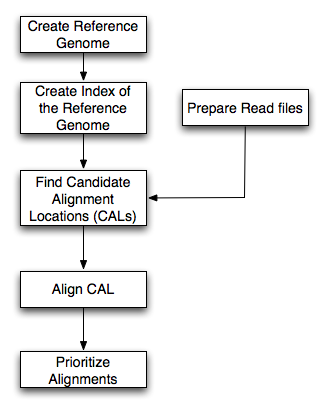
\includegraphics[scale=0.45]{figures/workflow.png} 
%
%\caption{\small Overall workflow for a mapping procedure using BFAST.  In this work, we focus on the step for finding Candidate Alignment Locations (CALs).  }
%  \label{fig:workflow-bfast} 
% \end{figure}
%
%
%\begin{table}
%\begin{tabular}{|c|c|c|c|} 
%  \hline 
% BFAST command & Description & Features for \\ 
%  &  &     Parallelism \\ \hline \hline
%\texttt{bfast fasta2brg} & creation of a ref. genome  &    multiple independent contigs \\ \hline 
%\texttt{solid2fastq}  &  preparation of short reads files &     multiple sequence reads files \\ \hline
%
%\texttt{bfast index} & creation of reference genome indexes& multi-threading and  \\
% &   & low memory option  \\  \hline
%\texttt{bfast match} & finding candidate alignment locations  &  multi-threading and  \\
%& &  parallel execution \\ \hline
%\texttt{bfast localalign} & alignment of each CAL  &   parallel execution \\  \hline
%\texttt{bfast postprocess} & prioritization of alignments  &  parallel execution \\ \hline
%
%
%\hline
%\end{tabular} \caption{Description of BFAST commands and features for parallel and multi-threading execution}
% \label{table:bfast-summary} 
%\end{table}
%

\subsection{TeraGrid Usage by the life science community}

The single largest community is the life-sciences community --
including MD (25\%)...
Get a break-down of the total usage of the TG by discipline and
application type.

\subsection{Large scale life science applications on the distributed HPC resources}

Traditionally, life science applications have been regarded as non-HPC applications.  Only a few applications were actively pursued in large scale computations.  Two representative examples are molecular simulations and virtual docking calculations.  For example, as the size of molecular system of interest grows and as the size of a chemical database for docking grows, the required computation needs to be scaled. Interestingly, while the former has advanced to be able to simulate larger systems with the so-called scale up of bulk synchronous techniques such as MPI, the latter has been pursued with many task computing strategies on clusters, HPC grids, and recently clouds.  

In spite of such conventional beliefs on life science applications, there has been striking progresses that appreciated the potential of large-scale distributed parallel executions.   For example, Next-Generation DNA Sequencing (hereafter, NGS) technologies challenge computational biology with unprecedented amounts of data produced by their high-throughput capability.  Required data analytics for processing such sequenced data along with dealing with genome data sets available in public and private databases is overwhelmed by the pace of growing data volume.  This poses the question on how the challenge of large volume data-management as well as the requirement of analyzing large volumes of data are effectively handled.  

Interestingly, the cyberinfrastructure considerations requried to
support a broad-range of analytical approaches and at the scales
required, has received less attention that the data-management problem
and algorithmic advances.  Thus not surprisingly, traditional
production cyberinfrastructure, such as the TeraGrid, have not been
used for such data-intensive analytics. There are multiple reasons,
but a couple of contributing factors are: (i) insufficient runtime
enviroments (and abstractions) to support concurrent computational
capabilties with large-data sets to support data-analytics (beyond
visualization) in an easy, scalable and extensible fashion, (ii)
insufficient support for user-customizable data-intensive "workflows"
that effectively hide the challenges of data-movement and efficient
data-management whilst managing concurrent distributed (computational)
resources.

Finally, traditional applications such as molecular simulations, virtual screening, and many bioinformatics applications, particularly, regarded as the non-HPC applications are dramatically enhanced by utilizing distributed scalable resources as we will show how a life science application benefits from the development of infrastructure to support a various execution patterns and the distributed data management with a user-friendly UI and other components to build a science gateway.

\subsection{Challenges in developing a gateway supporting heterogeneous HPC environments}



\section{Four Life Science Applications}

\begin{table}
\small
\begin{tabular}{|c|c|c|c|} 
  \hline Science Domain & Description & Target Application(s) 
  \\ \hline \hline 
  
  Molecular Dynamics &  &  \texttt{NAMD}  \\ \hline
  RNA Folding Prediction &  & \texttt{SFOLD, RNAFold} \\ \hline
  NGS data analytics &    &  \texttt{BFAST} \\ \hline
  Docking  &   & \texttt{Autodock} \\ \hline

\hline
\end{tabular} \caption{Four life science applications. The DARE framework was used for developing gateways for these applications}
 \label{table:four-applications} 
\end{table}

\textit{Large scale Molecular Dynamics simulations}
Over the past two decades, the field of biomolecular simulation has
exploded due to increases in computational power and parallel codes,
the emergence of accurate molecular mechanical potentials or force
fields and improvements in the methods~\cite{cheatham-1,
  cheatham-2}. A continually growing body of researchers apply
atomistic and coarse-grained molecular dynamics (MD) simulation
methods to facilitate drug discovery, perform advanced materials
research, to design and understand biomolecular and designed
catalysts, and to provide fundamental insight into molecular
structure, dynamics and interactions. Particular challenges include de
novo protein and nucleic acid folding and structure prediction;
correctly modeling induced-fit and conformational selection as drugs
or other molecules interact with a target macromolecule; modeling
large ensembles of biomolecules such as proteins in a membrane
environment, viruses, and biomolecular machines such as the ribosome;
combined quantum and molecular mechanical treatments for modeling
chemistry; and improving conformational sampling and estimation of
free energies and free energy pathways. 

In response to the perceived needs and importance of molecular
simulations, numerous high performance distributed memory parallel codes
have emerged in the past two decades (including NAMD~\cite{cheatham-3},
CHARMM~\cite{cheatham-4}, AMBER~\cite{cheatham-5},
LAMMPS~\cite{lammps}GROMACS~\cite{cheatham-6}, etc.), and many now can
directly include quantum representations. 

\textit{NGS-driven genome data analytics}

\textit{RNA structure prediction and beyond}


\textit{Drug Discovery via Docking strategies}

\subsection{Derive what the computational requirements and challenges
  for these applications are}
A growing limitation in the applications of life sciences is that workflow, data management, and
analysis have become rate limiting steps: what is missing is support for
the end-to-end execution requirement of applications.

We also need to move to tiered sets of computational resources.  For
example, one can imagine running large ensembles of MD engines on
tightly coupled parallel machines (like Ranger or Kraken) with
real-time data streamed to separately running analysis and
visualization resources (Lonestar, Spur), with on-the-fly monitoring
to analyze convergence, interesting phenomena or problems.  This also
provides the means for possible steering, for example by spawning or
stopping separate elements of the ensemble to sample more or less in a
particular region of interest.  In addition to real time monitoring,
hidden correlations in the data require the saving of coarser grained
simulation data on longer term (1-2 year) disk resources for further
analysis and mining using less tightly coupled computational
resources, and ultimately placing reduced and derived data sets
seamlessly back to the campuses, archivers, and for public
distribution.  Not only does this support the need for diverse sets of
computational resources, large-scale storage and data transfer
requirements for sophisticated analysis and visualization, and
high-bandwidth networking, it also drives the need for software tools
that facilitate the complicated workflow management, that allow
dynamic monitoring, starting and stopping of ensemble elements without
losing access to the global communications fabric and local
connections, and that provide the means for facilitating data
management and analysis.

In essence, the move from executing an individual task to \I{large
  ensembles} of coupled/loosely/uncoupled tasks requires scientists to spend
significant time on compute and data management problems, instead of
core science.  The quantitative shift (massive distributed parallel
compute and data resources) implies qualitative change in the way how life science applications are being served for scientific discovery. 

\jhanote{At the end we propose DARE based Gateways as a solution}


\section{Distributed Adaptive Runtime Environment}

\subsection{SAGA and BigJob abstraction}

To execute a scientific application using heterogeneous distributed computing resources, we develop the Distributed Adaptive Runtime Environment (DARE) framework\cite{dareurl}.  The framework is compose of an open source Web application framework, Pylons
and middleware of the application management system built upon SAGA an BigJob abstraction\cite{saga-ccgrid10,saga-royalsoc,saga-web,jha2009developing,ecmls10}.  This combination of the open source technology and the application management system enables us to develop a lightweight, extensible, full-fledged distributed computing science gateway quickly and effectively\cite{pylonsurl}. 

\subsection{Architecture}

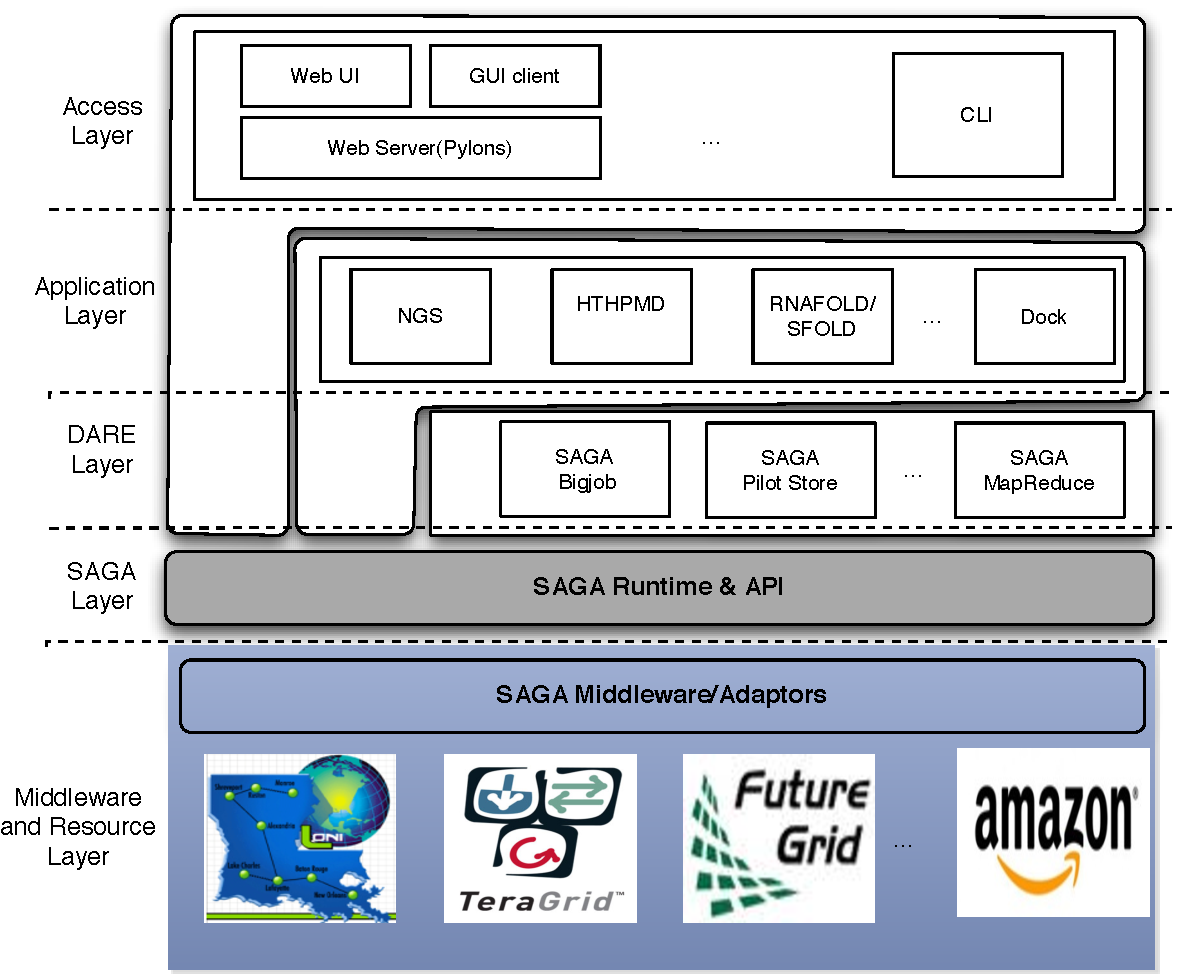
\includegraphics[scale=0.70]{figures/DAREOutline.pdf}

\subsection{The three components -- Access Layer, Services Layer and
  Resource/Provisioning Layer} 

Level 2: (i) Computational aspect, (ii) Data management and movement, 

Level 1: (iii)providing user interface

\section{Four DARE-based Gateways}
\subsection{DARE-NGS}
Our DARE-NGS gateway (http://cyder.cct.lsu.edu/dare-ngs) supports Genome-wide analysis on Teragrid and provides currently the mapping process using BFAST that aligns the large number of short reads sequenced from NGS machines onto a reference genome sequence, which is the first step in scientific discovery utilizing NGS sequencing-based protocols such as the whole genome resequencing, RNA-seq, and ChIP-seq.  De novo assembly without reference genome information is still in early stages.  Note that due to its design strategy, including other analysis tool such as assembly or extending to a pipeline with other tools successively applied after the mapping with DARE-NGS are straightforward and underway at this moment.

It is worth mentioning that the computational complexity
of the analysis (e.g. mapping) depends, upon other things, the size
and complexity of the reference genome and the data-size of short reads.
Given that these can vary significantly, the computational
requirements of NGS-analytics also varies (even between data-sets of
similar size).  Thus an efficient, scalable and extensible analytical
approaches must be supported by any framework supporting
NGS-analytics.

Recently, results of using DARE-NGS on the TeraGrid and
FutureGrid, using BFAST for mapping as the representative example of
the typical analysis that is required for NGS data were presented as a ECMLS11 (HPDC11) workshop paper.  

 \begin{table}
 \small
 \begin{tabular}{|c|c|c|c|c|c|c|c|c} 
 \hline 
 &  Type &Total     & $T_Q$ (S)          & $T_R$  (S)  & $T_{QR}$(S) &  $T_C$(S) & $T_{QRC}$ (S)  \\
 &          &Cores &  Queen Bee &  Ranger   &  Queen Bee &  Cloud &  Queen Bee,           \\
 &           &                        &                        &                   &  \&Ranger  &                &  Ranger \& Cloud \\       
 
  \hline
1 &  B. glumae   &   &                         &                   &   &                &    \\
\hline
2& HG18CHR21    & 64  &                         &                   &   &                &       \\
\hline
3 &  HG18    & 256  &   9586    &                   &   7582&                &      \\

\hline
\end{tabular}
\caption{  Time to completions in various cases  }
  
  \label{table:NGS-Distributed} 
\end{table}

\subsection{DARE-Rfold}


To support nc-RNA research and broadly for RNA structure prediction, with the science gateway, DARE-Rfold, a user is able to predict the Minimum Free Energy (MFE) secondary structure or an ensemble of structure sampled with a Boltzmann-weighted sampling scheme.  

Notably, many challenges in the computational investigation of RNA
folding dynamics exist.  For example, the support of high-throughput of highly-parallel tasks on heterogeneous distributed resources is critical.
We demonstrated the use of DARE-Rfold for the exploration of RNA folding energy landscape and structural characterization of SAM-I riboswitch sequences, which was greatly facilitated by the flexibility of our DARE framework and the capacity for many task computing to deal with 1000 structures from each sequence among 2910 sequences of SAM-I RAN family. 

\subsection{DARE-Dock}



\subsection{DARE-HTHP}






\subsection{How does this meet the requirements}
\smnote{ 1) Lets say we have "n" read files and with DARE it takes around time "t" time for matching step if we run it serially it would take n*t time. It probably exceeds wall time limit. Therefore speed up in match step depends how many number of read files we generate and process concurrently.
2) Yes we were able to process the complete run with entire Human Genome on QB and Ranger separately. (**I am currently working this to utilizing QB and Ranger together.) 
4) it should clearly provide the advantage with multiple resources. If we want to use the cloud resources from India to complete Human Genome run it is not practically possible because of the current limited disk size access provided by the FG Eucalyptus resources. Because whole human genome index files are of size 129 GB for Bfast matching step as opposed to HG 18 Chromosome 21 with size of  2 GB index files. On the other hand it also requires the temporary files disk space.  Thus it is important to utilize large capacity resources like QB and Ranger divide the work load across machines.}


\bibliographystyle{abbrv}
\bibliography{tg11}




\end{document}

